\chapter{実験}
\label{chap:evaluation}

% \section{装置幅}
% 分光器に単波長の光を入射させたとしても,スペクトルは収差やスリット幅に依存した有限の幅を持つ.
% この各分光器ごとに固有であるスペクトルの幅を装置幅と呼ぶ.
% ここではスペクトル形状をガウス関数でフィッティングした際の半値全幅を装置幅と定義する.
\section{実験概要}
% Fe-Neホローカソードランプを光源に波長範囲約400 nm~730 nmで対応する回折格子パルスを変えながら150個のデータを撮影した.
Fe-Neホローカソードランプを光源に回折格子パルスを8000から90ずつ大きくしていき21410まで変えながら150個のデータを撮影した.
これは波長範囲で約400~730 nmに対応する.
露光時間は3秒,y軸方向のビニングサイズを4に設定した.
配置したホローカソードランプとスリットの外観写真を図\ \ref{fig:lamp_slit}に示す.
\begin{figure}[htbp]
    \centering
    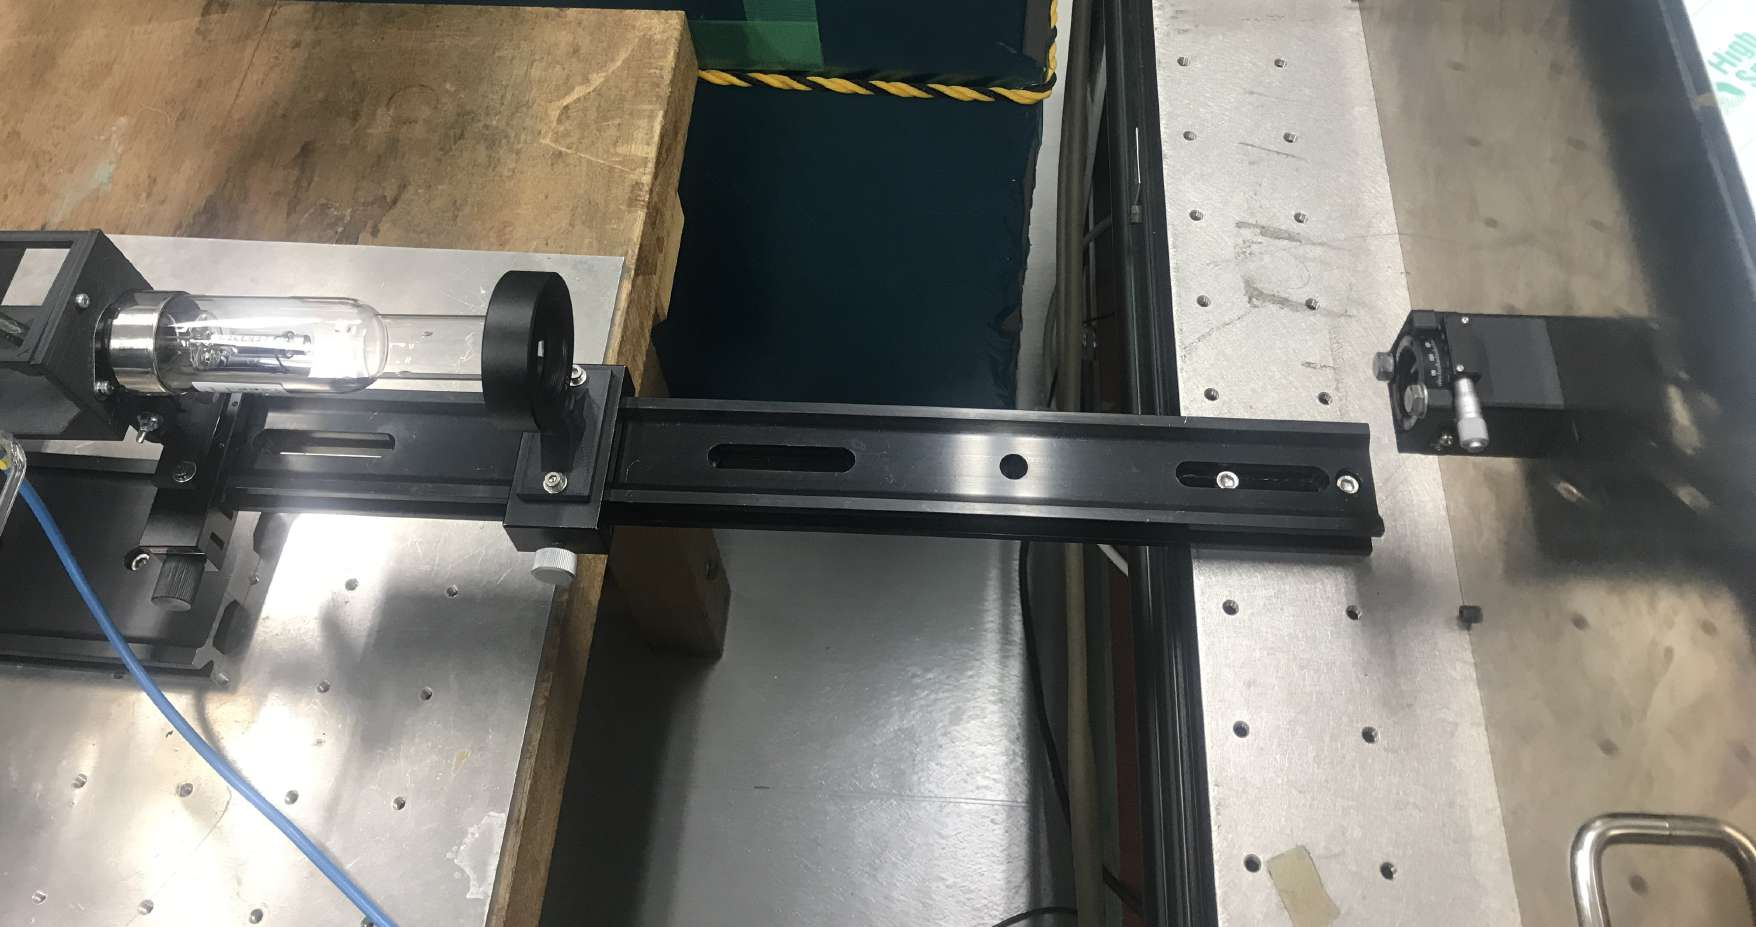
\includegraphics[scale=0.3]{figure/lamp_slit_compressed.pdf}
    \caption{Fe-Neホローカソードランプとスリットの配置の外観図}
    \label{fig:lamp_slit}
\end{figure}


ここで撮影した計測データの例として図\ \ref{fig:spectrum_example}に中心波長521.5 nmにおいて撮影されたCCDカメラ受光部の光の強度分布図を示す.
\begin{figure}[htbp]
    \centering
    \includegraphics[scale=1]{figure/spectrum_example.pdf}
    \caption{光源にFe-Neランプを用いて撮影した中心波長521.5 nmのCCDカメラ受光部の二次元光強度分布}
    \label{fig:spectrum_example}
\end{figure}
また図\ \ref{fig:spectrum_example2}は図\ \ref{fig:spectrum_example}の輝線部分(図\ \ref{fig:spectrum_example}におけるy軸方向に115~160ピクセル部分)の各ピクセルをy軸方向に平均しプロットした図である.
ここで縦軸は光の強度を表す.
\begin{figure}[htbp]
    \centering
    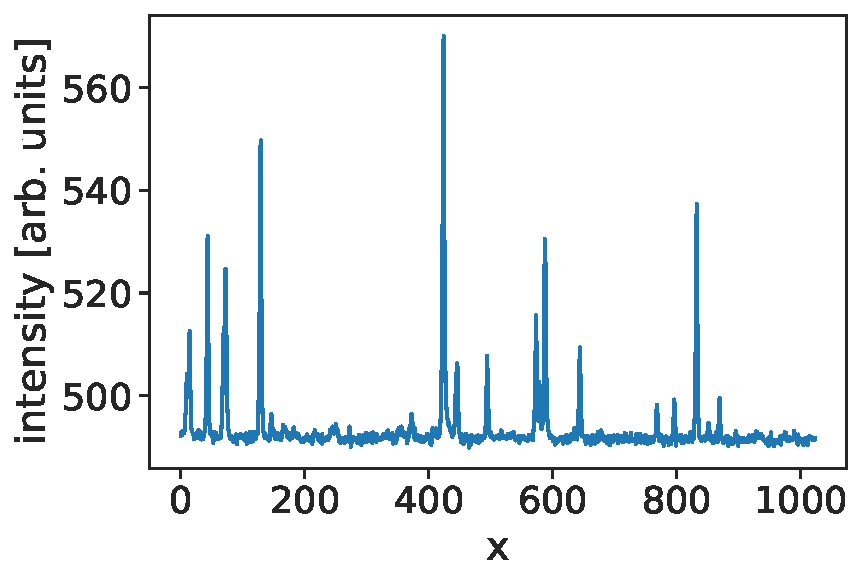
\includegraphics[scale=0.8]{figure/spectrum_example2.pdf}
    \caption{中心波長521.5 nmにおいて撮影したFeのスペクトル}
    \label{fig:spectrum_example2}
\end{figure}
撮影した150枚全てで図\ \ref{fig:spectrum_example2}のようなスペクトルを作成した.

\section{スペクトルの結合}
150枚のデータを撮影した際それぞれの隣り合うデータは一部が共通の波長領域になるように設定している.
そのため,150枚のスペクトル図は波長方向に一部を重ねて結合することができる.
ここで例として中心波長518.9 nmにおけるスペクトルと中心波長516.4 nmにおけるスペクトルを図\ \ref{fig:spectrum_example105},図\ \ref{fig:spectrum_example106}に示す.
\begin{figure}[htbp]
    \centering
    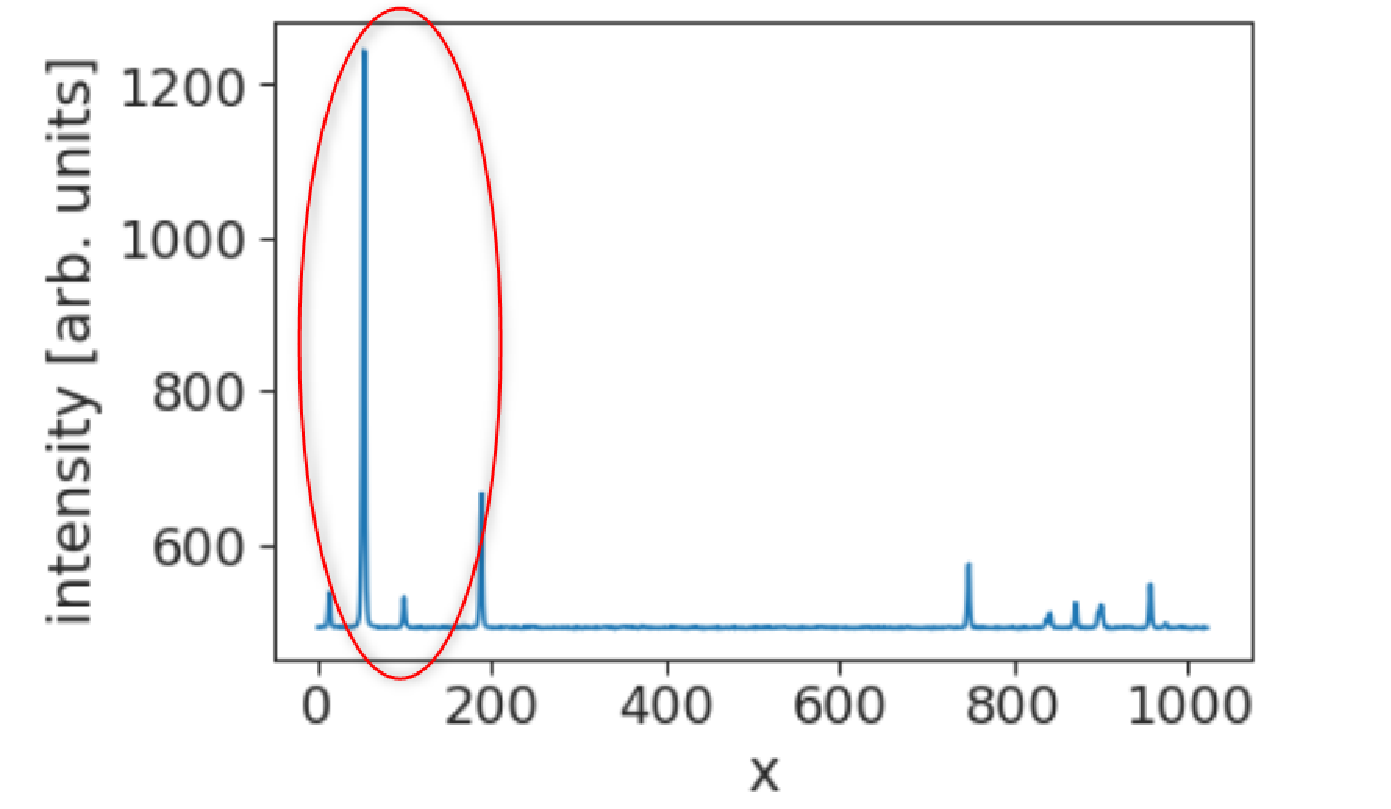
\includegraphics[scale=0.6]{figure/spectrum_example_105.pdf}
    \caption{中心波長518.9 nmにおけるスペクトル.赤く囲った部分が中心波長516.4 nmにおけるスペクトルと共通している.}
    \label{fig:spectrum_example105}
\end{figure}
\begin{figure}[htbp]
    \centering
    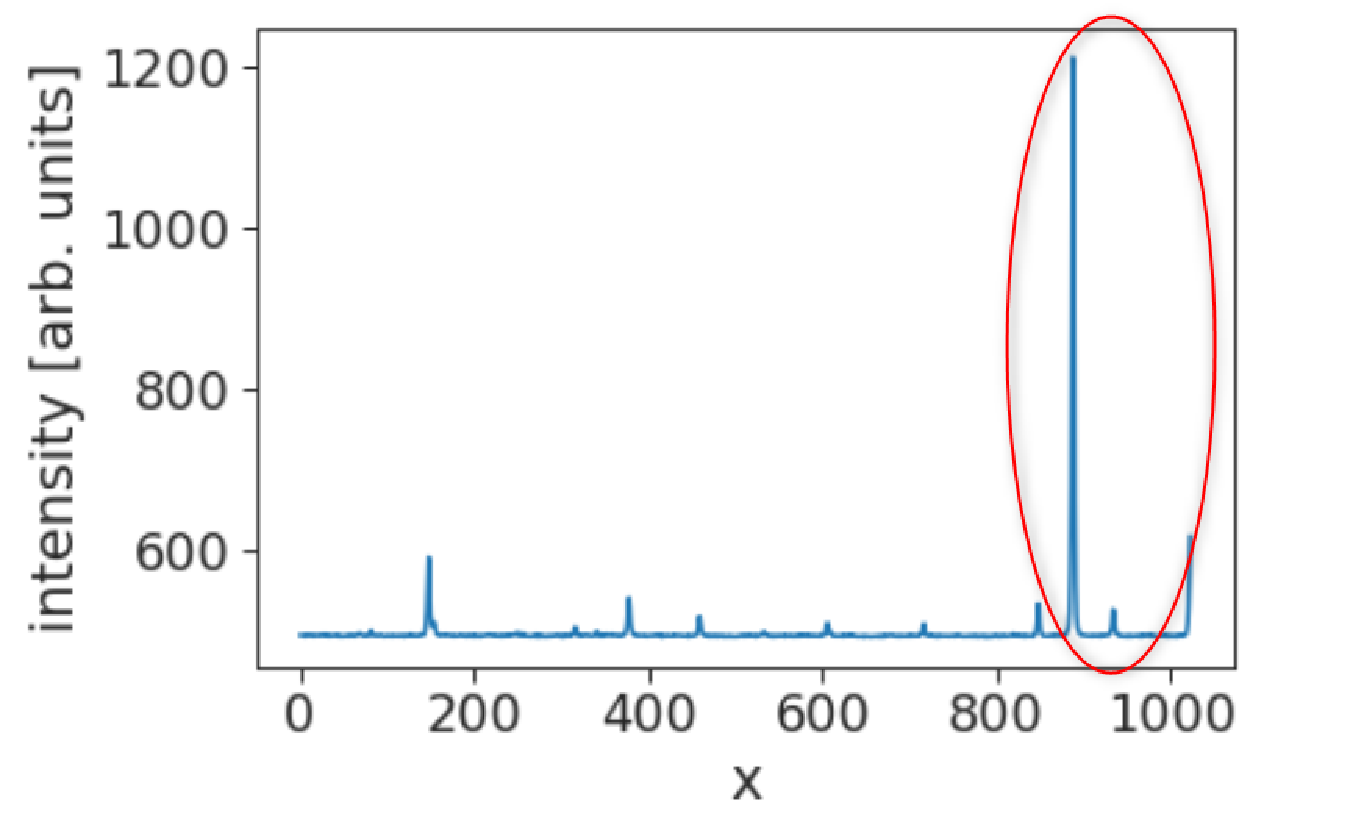
\includegraphics[scale=0.6]{figure/spectrum_example_106.pdf}
    \caption{中心波長516.4 nmにおけるスペクトル.赤く囲った部分が中心波長518.9 nmにおけるスペクトルと共通している.}
    \label{fig:spectrum_example106}
\end{figure}
赤線で囲まれた部分のスペクトルの形が一致していることからこの部分で同じ波長領域を観測していることが分かる.
重なり幅を調べるため相関係数を用いる.
中心波長518.9 nmにおけるスペクトルと中心波長516.4 nmにおけるスペクトルを$d$ピクセルだけ重ねた際の重なり部分における相関係数$r$を求め,$r$が1に最も近くなる$d$を調べた.
相関係数は以下の式で求められる.
\begin{equation}
     r = \frac{\frac{1}{d}\sum_{i=1}^{d} {(X_i-\overline{X})(Y_{1024-i+1}-\overline{Y})}}{{\sqrt{\frac{1}{d}\sum_{i=1}^{d} {(X_i-\overline{X})^2}}\times\sqrt{{\frac{1}{d}\sum_{i=1}^{d} {(Y_{1024-i+1}-\overline{Y})^2}}}}}
\end{equation}
ここで$\overline{X}$,$\overline{Y}$はそれぞれ$X$,$Y$の平均値である.
今回$X$は中心波長518.9 nmにおけるスペクトルの光の強度を,$Y$は中心波長516.4 nmにおけるスペクトルの光の強度を表す.
重なり幅$d$を変化させたときの相関係数$r$の変化の様子を図\ \ref{fig:correlation_coefficients}に示す.
\begin{figure}[htbp]
    \centering
    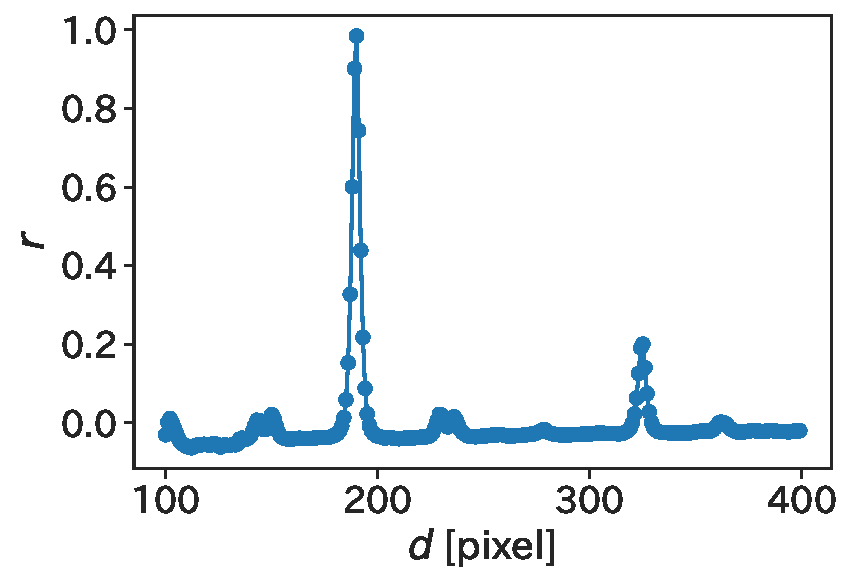
\includegraphics[scale=0.7]{figure/correlation_coefficients.pdf}
    \caption{重なり幅dを変化させたときの中心波長518.9 nmにおけるスペクトルと中心波長516.4 nmにおけるスペクトルの相関関数の変化}
    \label{fig:correlation_coefficients}
\end{figure}
図\ \ref{fig:correlation_coefficients}より中心波長518.9 nmにおけるスペクトルと中心波長516.4 nmにおけるスペクトルは190ピクセル分だけ重ねられることが分かった.
同様のことを他のスペクトルに対しても行い重なり幅を求め,全てのスペクトルを波長方向に結合した.

\section{波長校正}
4.3節の波長校正より150枚の各スペクトルの中心の波長を求めることができるが,これだけではそれぞれのピクセルにあるスペクトルの波長を求めることはできない.
ここで重ね合わせる前の各スペクトルの中心の波長を求め,線形補完することで各ピクセルの波長を求めた.
$n$枚目のスペクトルの$x=a$の波長($\lambda_{n,a}$)を表す式を以下に示す.
\begin{equation}
     \lambda_{n,a} = \lambda_n + \frac{(a-512)(\lambda_n-\lambda_{n+1})}{1024-d_n} 
\end{equation}
ここで$\lambda_n$は$n$枚目のスペクトルの中心波長,$d_n$は$n$枚目と$n+1$枚目のスペクトルの重なり幅を表す.
右辺第二項の分母$(1024-d_n)$は$n$枚目のスペクトルと$n+1$枚目のスペクトルを重ね合わせた時のそれぞれのスペクトルの中心間距離を表す.
$(a-512)$は$n$枚目のスペクトルにおける中心ピクセル$(x=512)$との距離を表す.
これによりスペクトルの横軸を波長に変換した.
150枚のスペクトルを結合させ,横軸を波長に変換した図が図\ \ref{fig:fe_wide_range}である.
\begin{figure}[htbp]
    \centering
    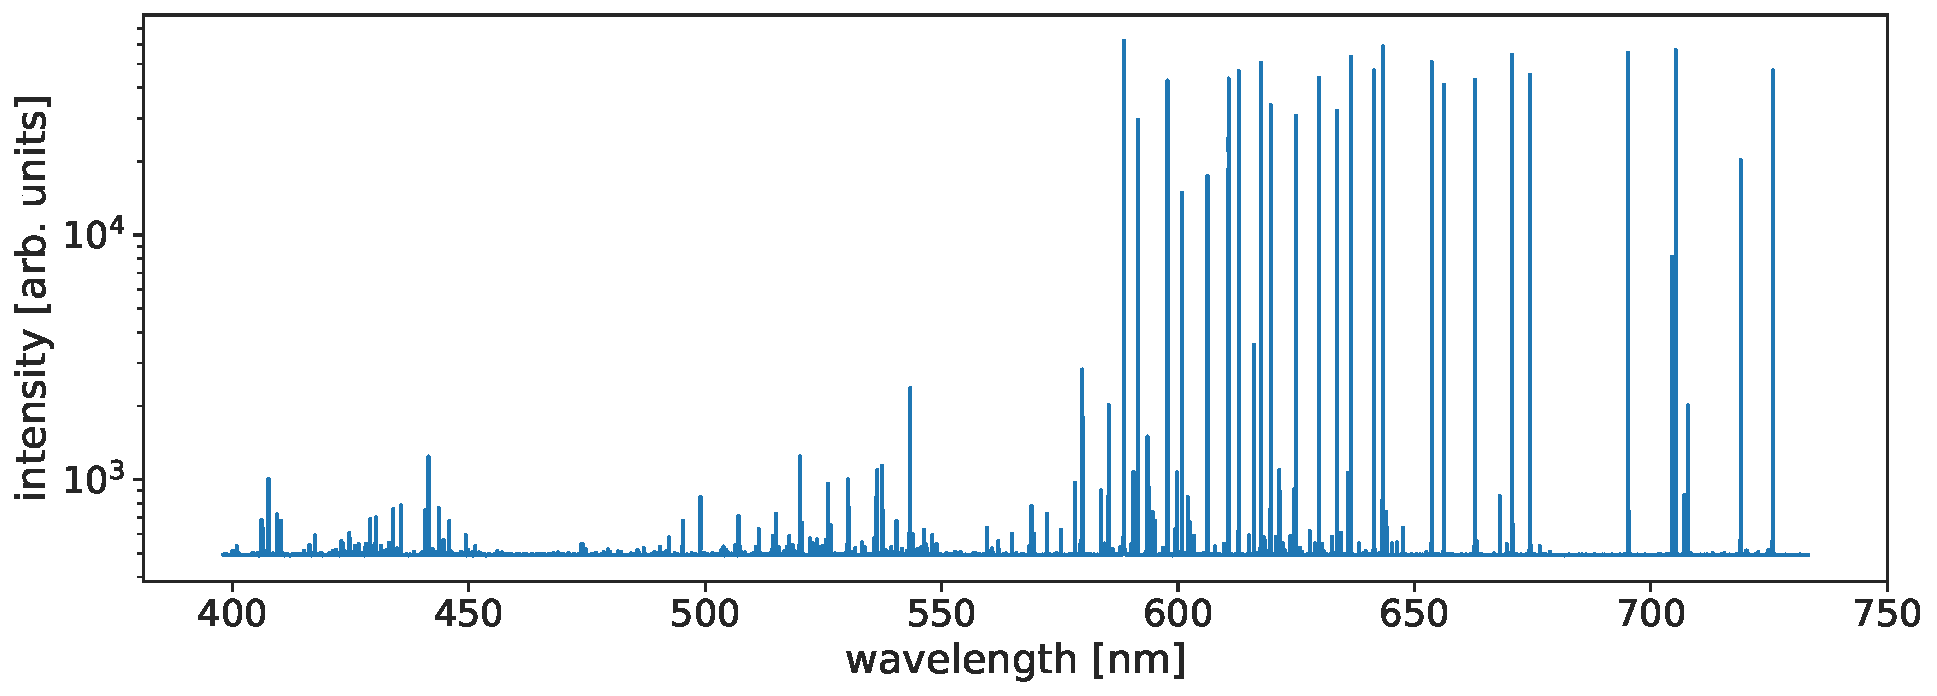
\includegraphics[scale=0.5]{figure/fe_wide_range.pdf}
    \caption{撮影した波長範囲でのFeのスペクトル(縦軸は対数目盛)}
    \label{fig:fe_wide_range}
\end{figure}
% また,Fig.\ \ref{fig:fe_wide_range}の光が低強度の部分を拡大したものがFig.\ \ref{fig:fe_wide_range_zoom}である.
% \begin{figure}[htbp]
    % \centering
    % 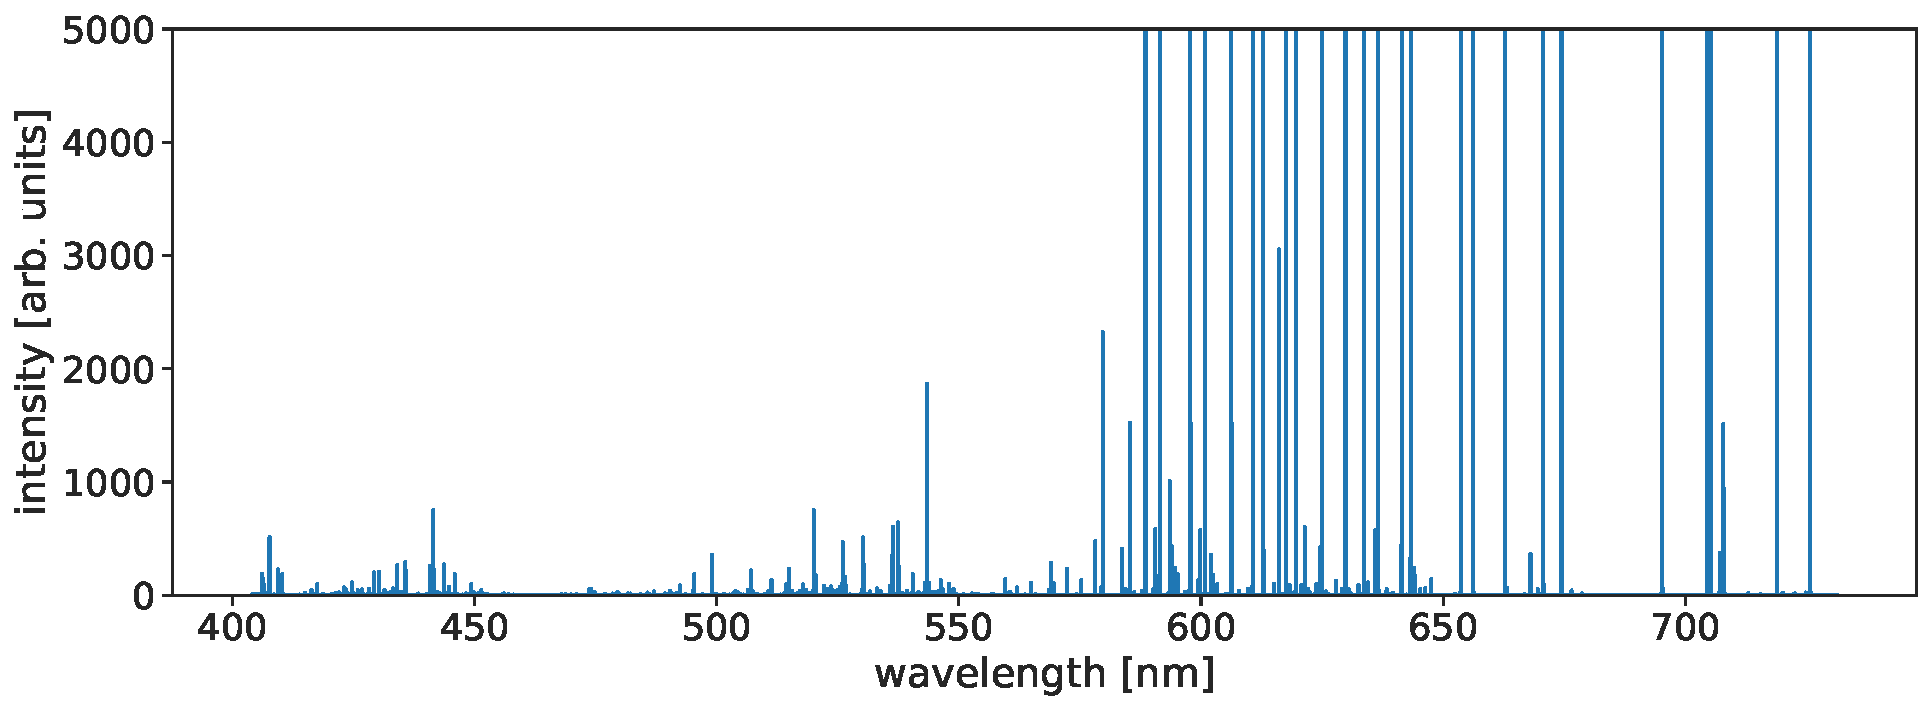
\includegraphics[scale=0.5]{figure/fe_wide_range_zoom.pdf}
    % \caption{Fig.\ \ref{fig:fe_wide_range}の光強度が小さい部分の拡大図}
    % \label{fig:fe_wide_range_zoom}
% \end{figure}
% 本研究で使用しているCCDカメラの情報処理容量は16bitであるため,各ピクセルにおいて$2^{16}-1=65535$までしか光の強度を表すことができない.
% Fig.\ \ref{fig:fe_wide_range}を見ると高波長側で強度が大きいスペクトルが存在する.

\section{装置幅}
% 分光器に単波長の光を入射させたとしても,スペクトルは収差やスリット幅に依存した有限の幅を持つ.
% この各分光器ごとに固有であるスペクトルの幅を装置幅と呼ぶ.
分光器に単色光を入射したときに得られるスペクトルをガウス関数でフィッティングした際の半値全幅を装置幅と定義する.
先ほど実験で用いたFe-Neホローカソードランプは装置幅以外の要因でのスペクトルの広がりは小さい.
そのため,本研究ではFeのスペクトルをガウス関数でフィッティングした際の半値全幅を装置幅とする.

本研究で使用しているCCDカメラは各ピクセルにおいて$2^{16}-1=65535$までしか光の強度を表すことができない.
飽和したピクセルは光の強度を正しく表すことができず,そのピクセルから作成されるスペクトルは正確な幅を求めることができない.
そこで今回は光の強度が50000以下のスペクトルを用いて装置幅を求める.
% ここで,Fig.\ \ref{fig:fe_wide_range}において強度の大きいスペクトルは飽和して信号電荷が上限値となっているピクセルを含んでいる可能性がある.
% このようなピクセルを使ってスペクトル図を作成すると幅を求める際に正確性が失われる.
% そのため,この強度の高いスペクトルはFeによる発光線ではなく封入ガスであるNeによる発光線を含んでいると考えた.
% 今回,装置幅を求めるために欲しいのはFeのスペクトルでありNeのスペクトルは不要である.
% また,装置幅を求めるためにはFig.\ \ref{fig:spectrum_example2}にあるほど多数のスペクトルは必要としておらず,S/N比の大きいスペクトルが全体で数十個あれば十分である.
% そこでFig.\ \ref{fig:fe_wide_range}に無数にあるピークの中から,装置幅を求めるのに使用するピークを抽出した.
% そのため,Fig.\ \ref{fig:fe_wide_range}のスペクトルから光の強度が150から40000のピークをピックアップし,これらを用いて装置幅を求めることとする.
装置幅を求めるのに使用するピークを抽出するためにPythonのパッケージであるscipyのfind\_peaks関数\cite{scipy}を用いた.
find\_peaks関数は高さなどの特性を指定して極大値を見つけ出す関数である.
装置幅を求めるために,図\ \ref{fig:fe_wide_range}のスペクトルから光の強度が200から50000のピークを抽出した.
抽出したピークを図\ \ref{fig:fe_wide_range_peak}に示す.
\begin{figure}[htbp]
    \centering
    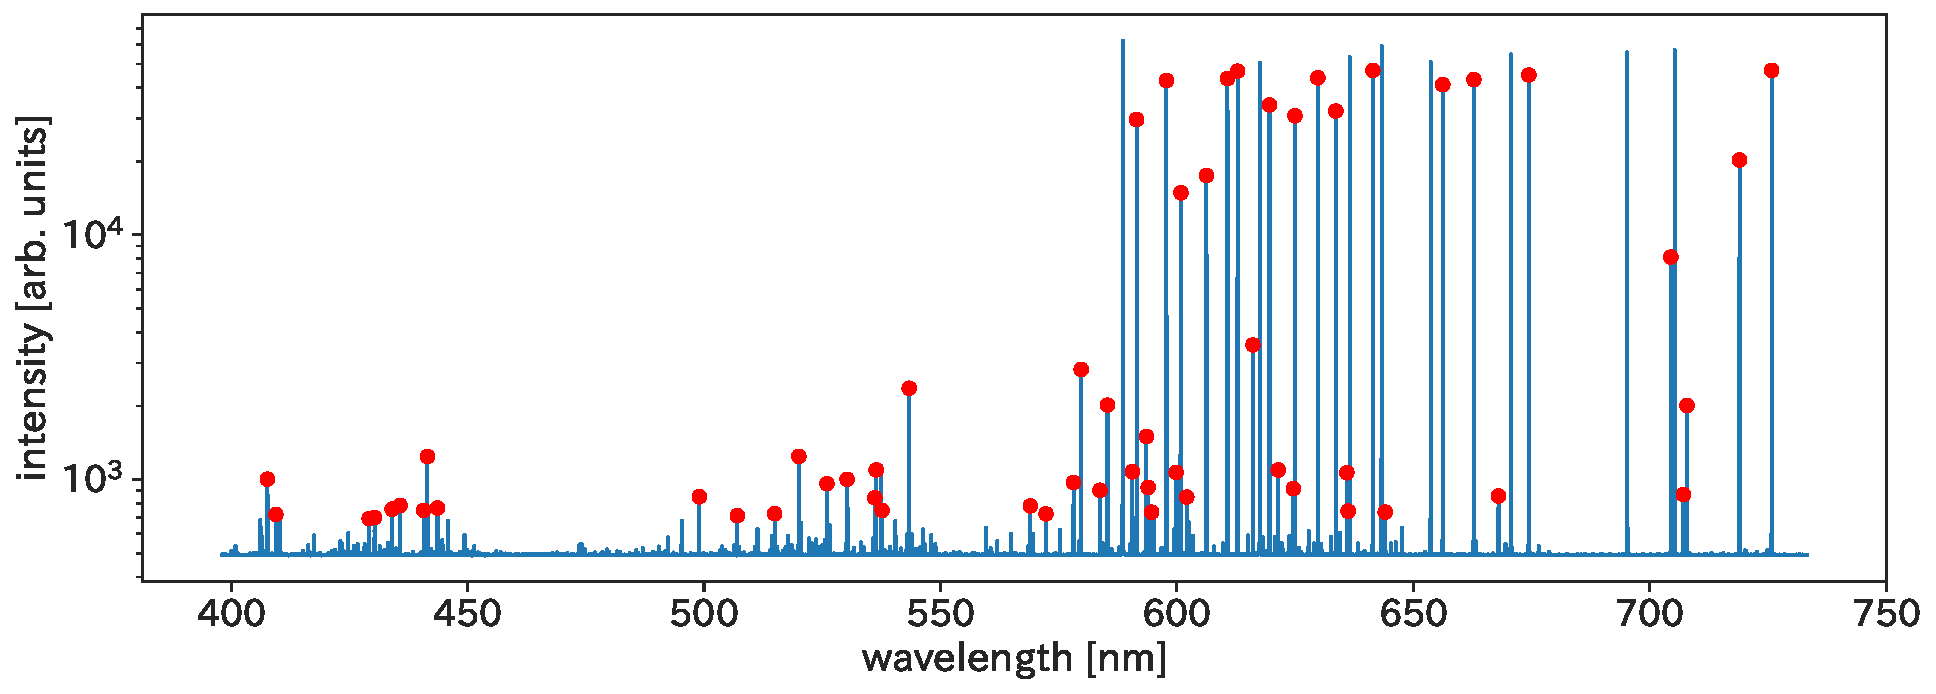
\includegraphics[scale=0.5]{figure/fe_wide_range_peak.pdf}
    \caption{装置幅を求めるために抽出したピーク点(赤丸)}
    \label{fig:fe_wide_range_peak}
\end{figure}
図\ \ref{fig:fe_wide_range_peak}の赤点をピークに持つスペクトルをそれぞれガウス関数でフィッティングし,半値全幅を求めた.
% Fig.\ \ref{fig:instrumental_function}は各スペクトルの半値全幅を波長に対してプロットしたものである.
% \begin{figure}[htbp]
%     \centering
%     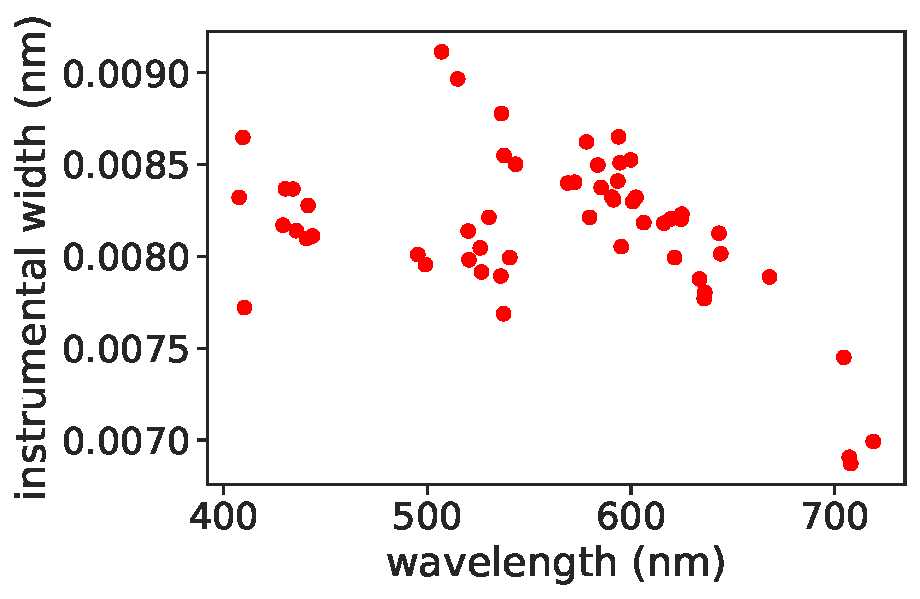
\includegraphics[scale=0.7]{figure/instrumental_function.pdf}
%     \caption{分光器装置幅の波長依存性}
%     \label{fig:instrumental_function}
% \end{figure}

\section{理論装置幅との比較}
図\ \ref{fig:instrumental_function_design}上に求めたスペクトルの半値全幅をプロットした(図\ \ref{fig:instrumental_function2}).
\begin{figure}[htbp]
    \centering
    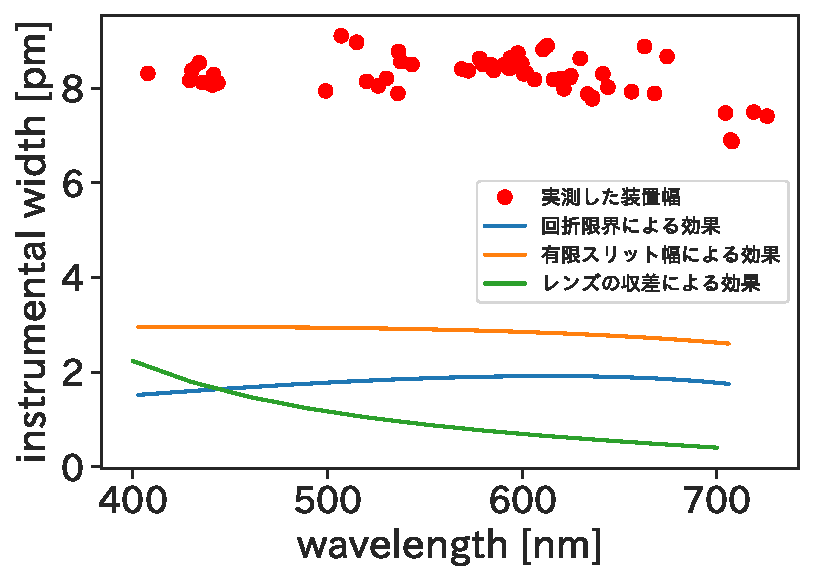
\includegraphics[scale=0.7]{figure/instrumental_function2.pdf}
    \caption{分光器装置幅と各条件での理論装置幅の比較}
    \label{fig:instrumental_function2}
\end{figure}
レンズの収差や回折限界による影響を受けないと仮定すると理論装置幅は3.0 pmほどになるが,実際の装置幅は波長に依存なく6.9~9.1 pmに分布していた.

% レンズが本来の性能通りに集光できていれば3.0 pmの装置幅は実現できるはずである.
% しかし,今回の測定ではレンズは理想通りにCCDカメラに対して結像できなかったため装置幅が大きくなってしまった.
レンズの集光性能が十分であるため理論装置幅を実現できると考えていたが,今回の計測において分光器は理論装置幅を実現することができなかった.
これは他の要因の影響を受けているためだと考えられるが,その要因についてはまだ判明しておらず今後の課題である.